\chapter{Mathematical and technical Fundamentals}
\label{chap:mathFund}


\section{3D-USCT}

The three dimensional ultra sonic computed tomography (3D-USCT) imaging technique is a promising rather new technique for the detection of breast cancer in early stages \cite{Ruiter2011RealizationUSCT}.

The second version prototype of the 3D-\ac{usct} can be seen in figure \ref{usct_example}. On the left the picture shows the patient bed with the aperture for the breast. The patient has to lie down on their stomach during the imaging procedure. The breast will be placed in the water-filled semi-ellipsoidal aperture which can be seen on the lower right side of the figure. On the top-right of figure \ref{usct_example} the aperture is visible with over 2000 US-transducers.
For the examination the patient has to lie down on a bed with an semi-ellipsoidal aperture for the breasts and has to remain still to avoid image degradation \cite{Ruiter2011RealizationUSCT}. 

To measure the pressure over time the prototype of the \ac{usct} at the KIT comprises 628 emitting and 1413 receiving transducers fitted into the wall of the aperture. The aperture itself has a height of 17cm and diameter of 26cm \cite{Kretzek2014GPUAberration}.

During each scan one transducer acts as an emitter whereas all the other transducers are receiving the signal. For every emitter-receiver combination a so called \ac{ascan} is recorded. Each \ac{ascan} comprises the progression of the pressure at the transducer which is plotted over the time. After each emitter-receiver combination was recorded the aperture is rotated to compensate the gaps between each \ac{tas}. In total there are ten positions for which each emitter-receiver scan is repeated.
 


\begin{figure}[H]
    \centering
    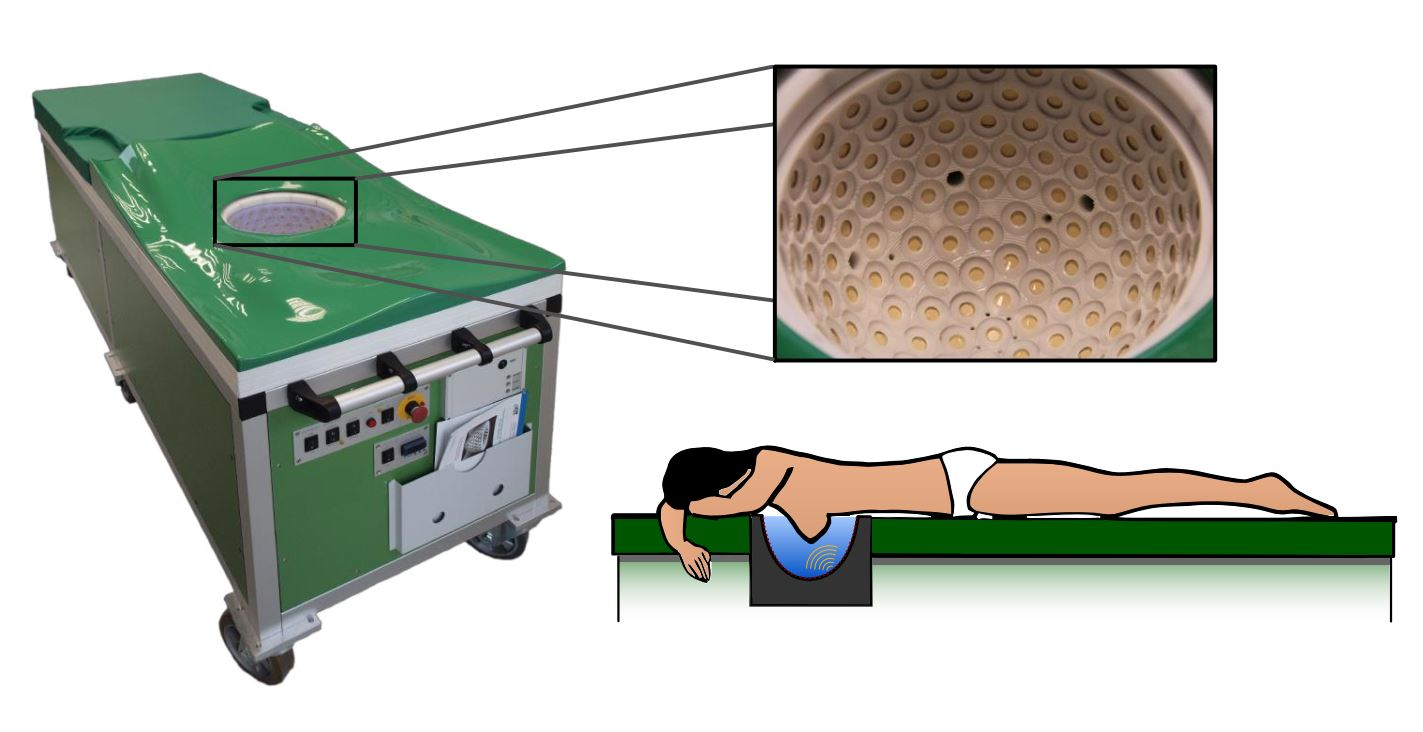
\includegraphics[width=1\textwidth]{usct_schematic.jpg}
    \caption{The prototype of an 3D-\ac{usct} at the KIT research facility. Picture source: \cite{Kretzek2014GPUAberration}. }
    \label{usct_example}
\end{figure}


For the generation of the final image so far three different modalities are used. 


- aperture rotation
- techniqual aspects
- pumps
- computer
- data processing




\section{Characterisation of reflections}


\section{Platonic geometries}
\subsection{Gradnetz}


\section{Spherical coordinate system}
Spherical coordinates are used to create an arbitrary amount of normal vectors to characterise the different directions for each voxel. Depending on the available computation power and memory it is possible to create as many normals as possible to cover as many possible directions as possible.


\subsection{Spherical coordinate system in 3D}

In three dimensions the spherical coordinate system consists of a radius $r$, and inclination $\vartheta$ and an azimuth $\varphi$. The conversion from one coordinate systems to the other can be seen in tables \ref{table_pol_to_cart} and \ref{table_cart_to_Pol}.

\begin{figure}[H]
  \centering
  \begin{minipage}[b]{0.45\textwidth}
    \centering
  \fbox{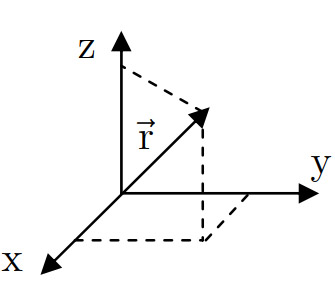
\includegraphics[width=0.75\linewidth]{cartesian_coord.jpg}}
  \caption{Cartesian coordinate system \cite{Prof.Dr.-Ing.GertF.Trommer2013FelderWellen}.}
  \end{minipage}
  \hfill
  \begin{minipage}[b]{0.45\textwidth}
    \centering
  \fbox{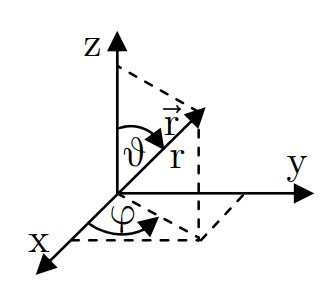
\includegraphics[width=0.75\textwidth]{polar_coord.jpg}}
  \caption{Spherical coordinate system \cite{Prof.Dr.-Ing.GertF.Trommer2013FelderWellen}.}
  \end{minipage}
    \hfill
\label{polar_cart_systems}
\end{figure}




\begin{table}[H]
\centering
\begin{tabular}{|ll|}
\hline
\textbf{Cartesian coordinate system} & \textbf{Spherical coordinate system}                                                                            \\ \hline
$x $                            & $= r \cdot sin(\vartheta) \cdot cos(\varphi)$ \\
$y $                            & $= r \cdot sin(\vartheta) \cdot sin(\varphi)$ \\
$z $                            & $= r \cdot cos(\vartheta)$                                                  \\ \hline
\end{tabular}
\caption{Conversion of polar coordinates to Cartesian coordinates  \cite{Bronstein2005TaschenbuchMathematik}.}
\label{table_pol_to_cart}
\end{table}


\begin{table}[H]
\centering
\begin{tabular}{|ll|}
\hline
\textbf{Cartesian coordinate system} & \textbf{Spherical coordinate system}                                                                            \\ \hline
$\sqrt{x^2+y^2+z^2} $                               & $= r$ \\
$arctan( \frac{\sqrt{x^2+y^2}}{z} ) $  & $= \vartheta$ \\ 
$arctan( \frac{y}{x} ) $               & $= \varphi$                                                  \\ \hline
\end{tabular}
\caption{Conversion of Cartesian coordinates to polar coordinates \cite{Bronstein2005TaschenbuchMathematik}. }
\label{table_cart_to_Pol}
\end{table}







\section{Graphic processing unit (GPU)}












\section{Speed of Sound correction}
\label{sec:sos_correct}
In the early stages of the project the speed of sound (SOS) for the calculation of the \ac{tof} in each \ac{ascan} was assumed to be constant for the whole path for the whole \ac{ascan}. Then the \ac{sos} was approximated to match the propagation velocity of a sound wave in water: $SOS_{path} \approx  \bar{c}_{water}$ \cite{Kretzek2014GPUAberration}.

Since this is only a very rough approximation of the actual \ac{sos} in the volume the assumption of a constant propagation velocity led to a reduced contrast in the reconstructed image as the real location of the scattering was blurred during this process.
To improve the contrast of the final image for each path the \ac{sos} is calculated. With Bresenhams line drawing algorithm \cite{Bresenham2010AlgorithmPlotter} the appropriate voxels along the path from the emitter to the scattering voxel and further to the receiver are selected. For each of these $N$ visited voxels the local velocity $c(\overrightarrow {x_k})$ is taken from the \ac{sos}-image from the preceding \ac{sos} measurement of the tissue.

The average velocity of the sound propagation for that certain path $\overline{SOS}_{path}$ then can be calculated with the harmonic mean in equation \ref{path_sos} \cite{Kretzek2014GPUAberration}:

\begin{equation}
 \overline{SOS}_{path} = \frac{N}{\sum_{k=1}^{N}  \frac{1}{c(\overrightarrow {x_k})} } 
\label{path_sos}
\end{equation}

During the \ac{saft} in equation \ref{eqation_tof} and \ref{eqation_Voxel_value} the \ac{sos} can be replaced by the much more realistic $\overline{SOS}_{path}$ for each individual propagation path.








\section{Arithmetic mean vs Harmonic mean}




